\documentclass[finnish,english,t]{beamer}
%\documentclass[finnish,english,handout]{beamer}

% Uncomment if want to show notes
% \setbeameroption{show notes}

\mode<presentation>
{
  \usetheme{Warsaw}
}
\setbeamertemplate{itemize items}[circle]
\setbeamercolor{frametitle}{bg=white,fg=navyblue}


% \usepackage[pdftex]{graphicx}
\usepackage[T1]{fontenc}
\usepackage[utf8]{inputenc}
\usepackage{times}
\usepackage{microtype}
\usepackage{epic,epsfig}
\usepackage{subfigure,float}
\usepackage{amsmath,amsfonts,amssymb}
\usepackage{inputenc}
\usepackage{babel}
\usepackage{afterpage}
\usepackage{url}
\urlstyle{same}
\usepackage{amsbsy}
\usepackage{eucal}
\usepackage{rotating}
\usepackage{listings}
\usepackage{lstbayes}

\usepackage{natbib}
\bibliographystyle{apalike}

% \definecolor{hutblue}{rgb}{0,0.2549,0.6784}
% \definecolor{midnightblue}{rgb}{0.0977,0.0977,0.4375}
% \definecolor{hutsilver}{rgb}{0.4863,0.4784,0.4784}
% \definecolor{lightgray}{rgb}{0.95,0.95,0.95}
% \definecolor{section}{rgb}{0,0.2549,0.6784}
% \definecolor{list1}{rgb}{0,0.2549,0.6784}
 \definecolor{navyblue}{rgb}{0,0,0.5}
\renewcommand{\emph}[1]{\textcolor{navyblue}{#1}}
\definecolor{darkgreen}{rgb}{0,0.3922,0}

\graphicspath{{./figs/}}

\pdfinfo{
  /Title      (Bayesian data analysis, ch 12)
  /Author     (Aki Vehtari) %
  /Keywords   (Bayesian probability theory, Bayesian inference, Bayesian data analysis)
}


\parindent=0pt
\parskip=8pt
\tolerance=9000
\abovedisplayshortskip=2pt

\setbeamertemplate{navigation symbols}{}
\setbeamertemplate{headline}[default]{}
\setbeamertemplate{headline}[text line]{\insertsection}
\setbeamertemplate{footline}[frame number]


\def\o{{\mathbf o}}
\def\t{{\mathbf \theta}}
\def\w{{\mathbf w}}
\def\x{{\mathbf x}}
\def\y{{\mathbf y}}
\def\z{{\mathbf z}}

\def\eff{\mathrm{eff}}
\def\ESS{\mathrm{ESS}}

\DeclareMathOperator{\E}{E}
\DeclareMathOperator{\Var}{Var}
\DeclareMathOperator{\var}{var}
\DeclareMathOperator{\Sd}{Sd}
\DeclareMathOperator{\sd}{sd}
\DeclareMathOperator{\Gammad}{Gamma}
\DeclareMathOperator{\Invgamma}{Inv-gamma}
\DeclareMathOperator{\Bin}{Bin}
\DeclareMathOperator{\Negbin}{Neg-bin}
\DeclareMathOperator{\Poisson}{Poisson}
\DeclareMathOperator{\Beta}{Beta}
\DeclareMathOperator{\logit}{logit}
\DeclareMathOperator{\N}{N}
\DeclareMathOperator{\U}{U}
\DeclareMathOperator{\BF}{BF}
\DeclareMathOperator{\Invchi2}{Inv-\chi^2}
\DeclareMathOperator{\NInvchi2}{N-Inv-\chi^2}
\DeclareMathOperator{\InvWishart}{Inv-Wishart}
\DeclareMathOperator{\tr}{tr}
% \DeclareMathOperator{\Pr}{Pr}
\def\euro{{\footnotesize \EUR\, }}
\DeclareMathOperator{\rep}{\mathrm{rep}}


\title[]{Bayesian data analysis}
\subtitle{}

\author{Aki Vehtari}

\institute[Aalto]{}

\begin{document}

\begin{frame}

  {\Large\color{navyblue} Chapter 12}

  \begin{itemize}
  \item {\color{gray} 12.1 Efficient Gibbs samplers (not part of the course)}
  \item {\color{gray} 12.2 Efficient Metropolis jump rules (not part of the course)}
  \item {\color{gray} 12.3 Further extensions to Gibbs and Metropolis (not part of the course)}
  \item 12.4 Hamiltonian Monte Carlo (important)
  \item 12.5 Hamiltonian dynamics for a simple hierarchical model (useful example)
  \item 12.6 Stan: developing a computing environment (useful intro)
  \end{itemize}
\end{frame}

\begin{frame}

  {\Large\color{navyblue} Extra material for dynamic HMC}

  \begin{itemize}
  \item Michael Betancourt (2018).  A Conceptual Introduction to
    Hamiltonian Monte Carlo. \url{https://arxiv.org/abs/1701.02434}
  \item Cole C. Monnahan, James T. Thorson, and Trevor A. Branch
    (2016) Faster estimation of Bayesian models in ecology using
    Hamiltonian Monte Carlo. \url{https://dx.doi.org/10.1111/2041-210X.12681}
  \item Michael Betancourt (2018). Scalable Bayesian Inference with
    Hamiltonian Monte Carlo
    \url{https://www.youtube.com/watch?v=jUSZboSq1zg}
  \end{itemize}

\end{frame}

\begin{frame}

  {\Large\color{navyblue} Extra material for Stan}

  \begin{itemize}
  \item Andrew Gelman, Daniel Lee, and Jiqiang Guo (2015) Stan: A
    probabilistic programming language for Bayesian inference and
    optimization. \url{http://www.stat.columbia.edu/~gelman/research/published/stan_jebs_2.pdf}
  \item Carpenter et al (2017). Stan: A probabilistic programming
    language. Journal of Statistical Software
    76(1). \url{https://dox.doi.org/10.18637/jss.v076.i01}
  \item Stan User's Guide, Language Reference Manual, and Language
    Function Reference (in html and pdf)
    \url{https://mc-stan.org/users/documentation/}
    \begin{itemize}
    \item[-] easiest to start from Example Models in User's guide
    \end{itemize}
  \item Basics of Bayesian inference and Stan, part 1 Jonah Gabry \&
    Lauren Kennedy (StanCon 2019 Helsinki tutorial)
    \begin{itemize}
    \item[-]
      \url{https://www.youtube.com/watch?v=ZRpo41l02KQ&index=6&list=PLuwyh42iHquU4hUBQs20hkBsKSMrp6H0J}
    \item[-] \url{https://www.youtube.com/watch?v=6cc4N1vT8pk&index=7&list=PLuwyh42iHquU4hUBQs20hkBsKSMrp6H0J}
  \end{itemize}
  \end{itemize}
\end{frame}


\begin{frame}

  {\Large\color{navyblue} Chapter 12 demos}

  \begin{itemize}
  \item demo12\_1: HMC
  \item \url{http://elevanth.org/blog/2017/11/28/build-a-better-markov-chain/}
  \item rstan\_demo
  \item rstanarm\_demo
  \item \url{http://sumsar.net/blog/2017/01/bayesian-computation-with-stan-and-farmer-jons/}
  \item \url{http://mc-stan.org/documentation/case-studies.html}
  \item \url{https://cran.r-project.org/package=rstan}
  \item \url{https://cran.r-project.org/package=rstanarm}
  \end{itemize}
  
\end{frame}

\begin{frame}

  {\Large\color{navyblue} Hamiltonian Monte Carlo}

  \vspace{-0.5\baselineskip}
  \begin{itemize}
  \item Uses log density (negative log density is called energy)
  \item Uses gradient of log density for more efficient sampling
  \item Augments parameter space with momentum variables
  \end{itemize}
  \vspace{-0.5\baselineskip}
  \only<1>{\phantom{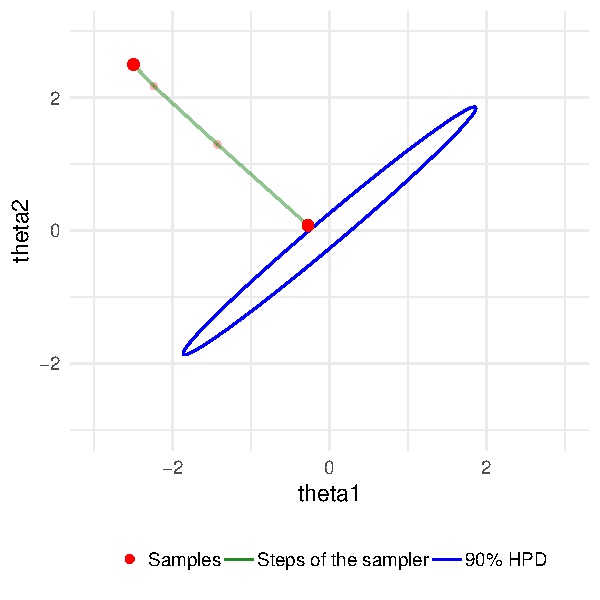
\includegraphics[width=9cm]{hmcdemo01.pdf}}}
  \only<2>{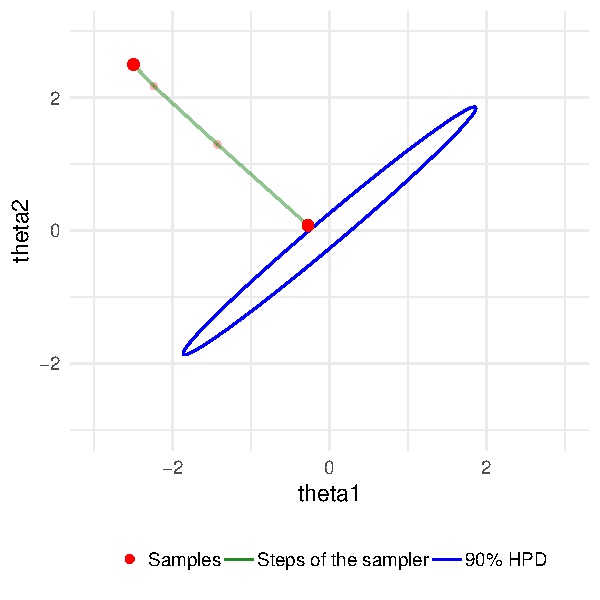
\includegraphics[width=9cm]{hmcdemo01.pdf}}
  \only<3>{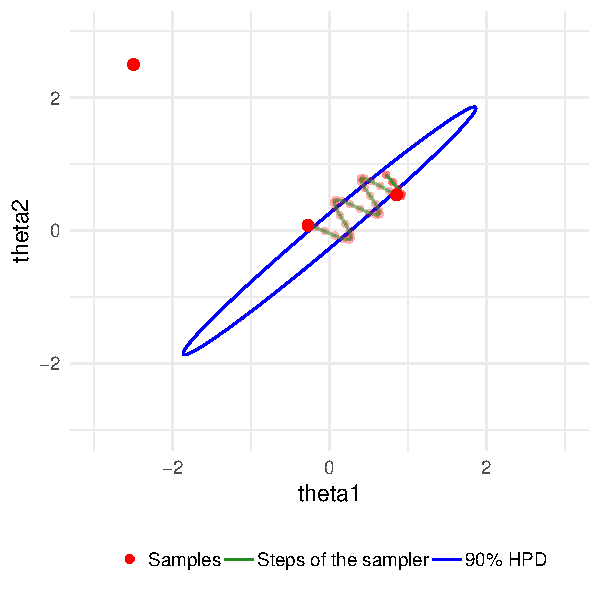
\includegraphics[width=9cm]{hmcdemo02.pdf}}
  \only<4>{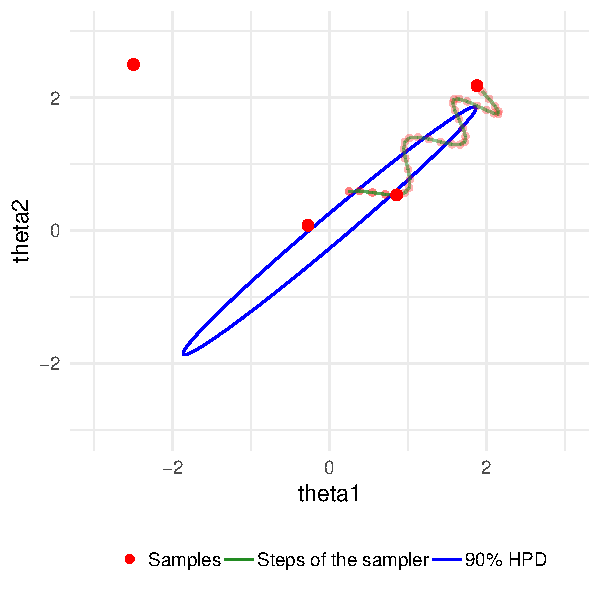
\includegraphics[width=9cm]{hmcdemo03.pdf}}
  \only<5>{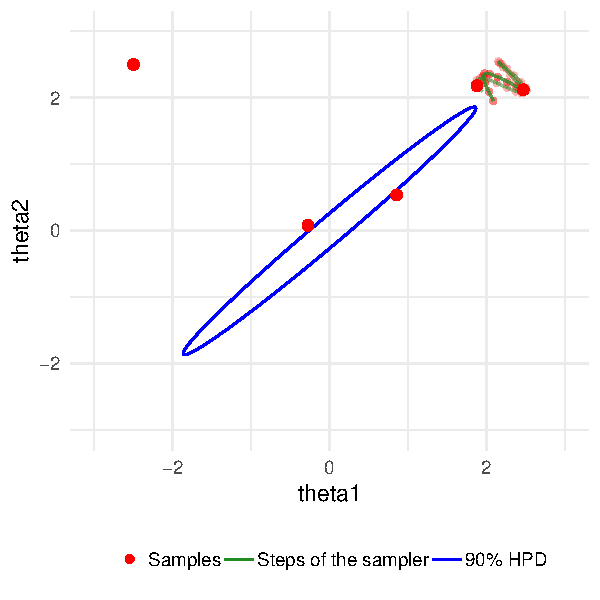
\includegraphics[width=9cm]{hmcdemo04.pdf}}
  \only<6>{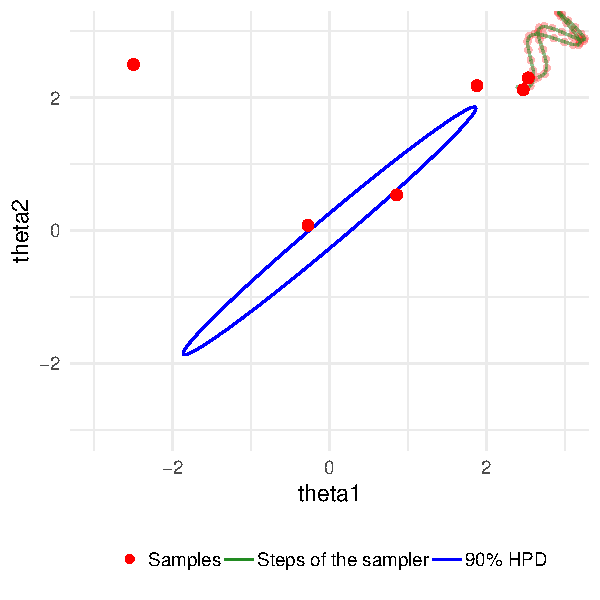
\includegraphics[width=9cm]{hmcdemo05.pdf}}
  \only<7>{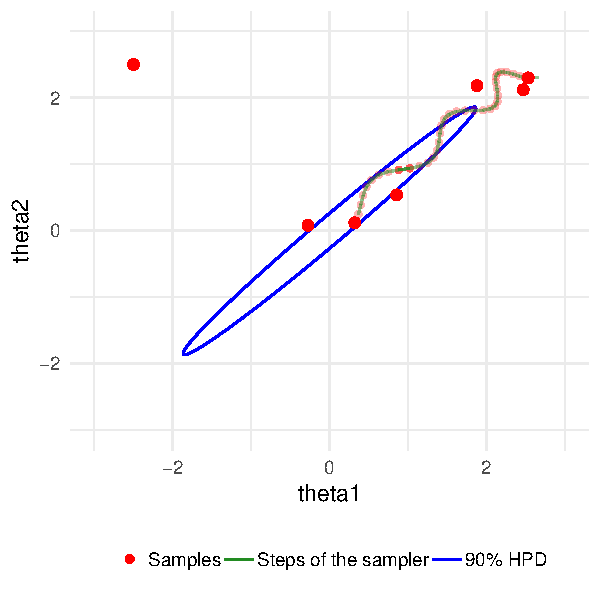
\includegraphics[width=9cm]{hmcdemo06.pdf}}
  \only<8>{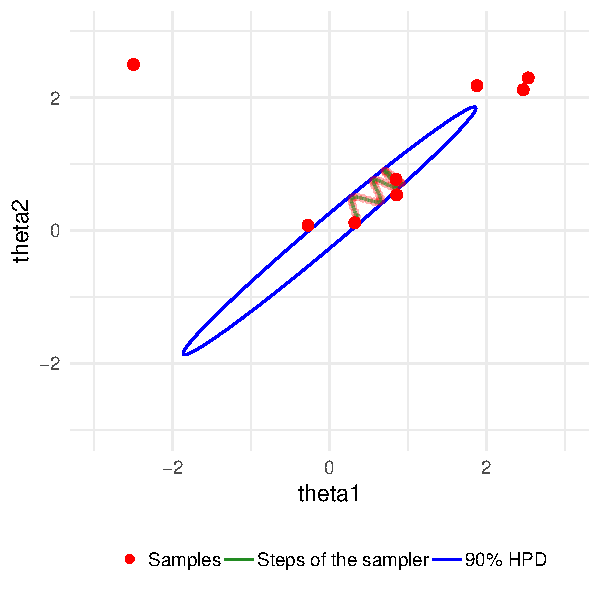
\includegraphics[width=9cm]{hmcdemo07.pdf}}
  \only<9>{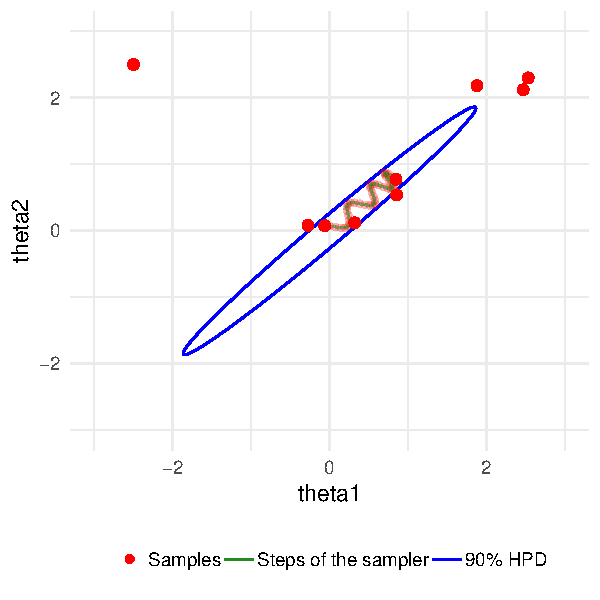
\includegraphics[width=9cm]{hmcdemo08.pdf}}
  \only<10>{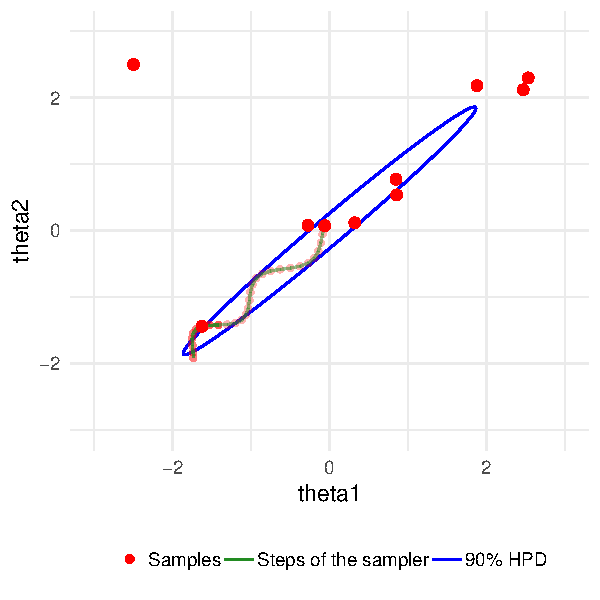
\includegraphics[width=9cm]{hmcdemo09.pdf}}
  \only<11>{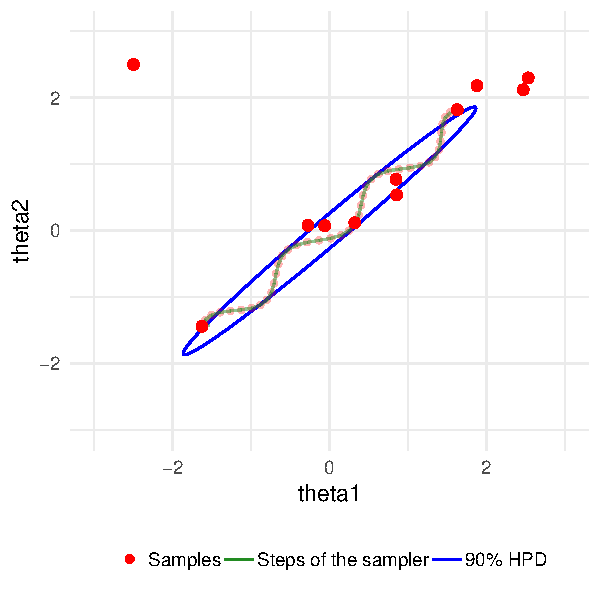
\includegraphics[width=9cm]{hmcdemo10.pdf}}
  \only<12>{\hspace{-5mm}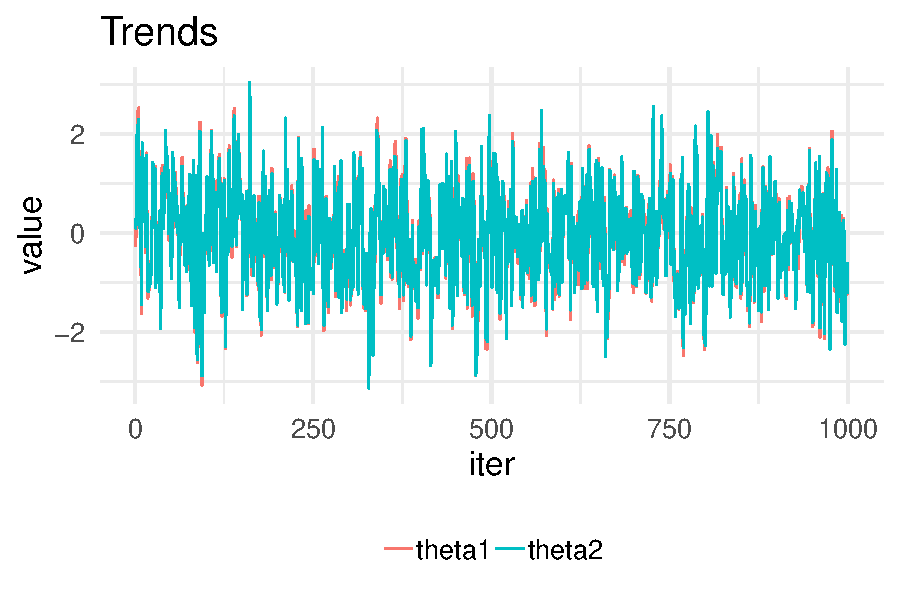
\includegraphics[width=12cm]{hmc1trace.pdf}}
  \only<13>{\hspace{-5mm}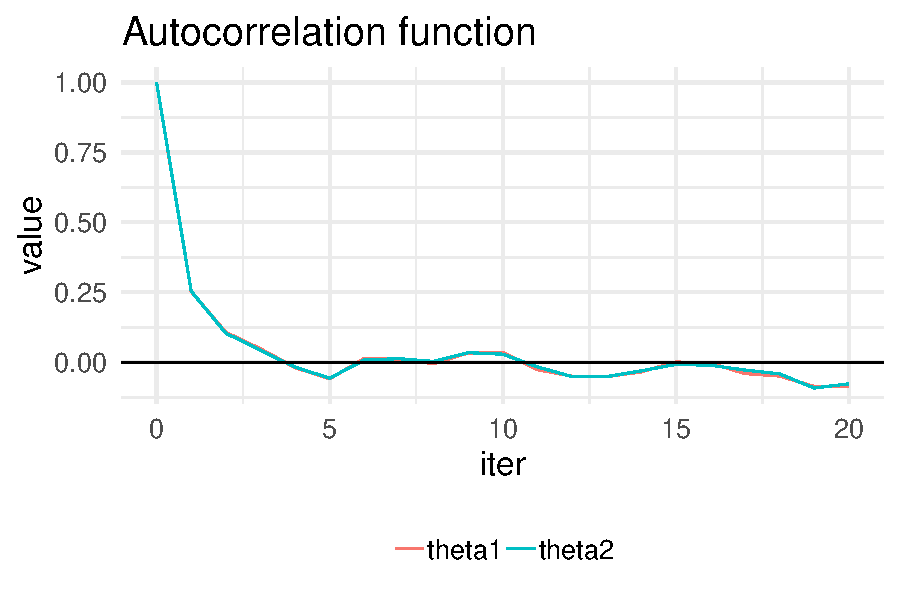
\includegraphics[width=12cm]{hmc1acf.pdf}}
  \only<14>{\hspace{-5mm}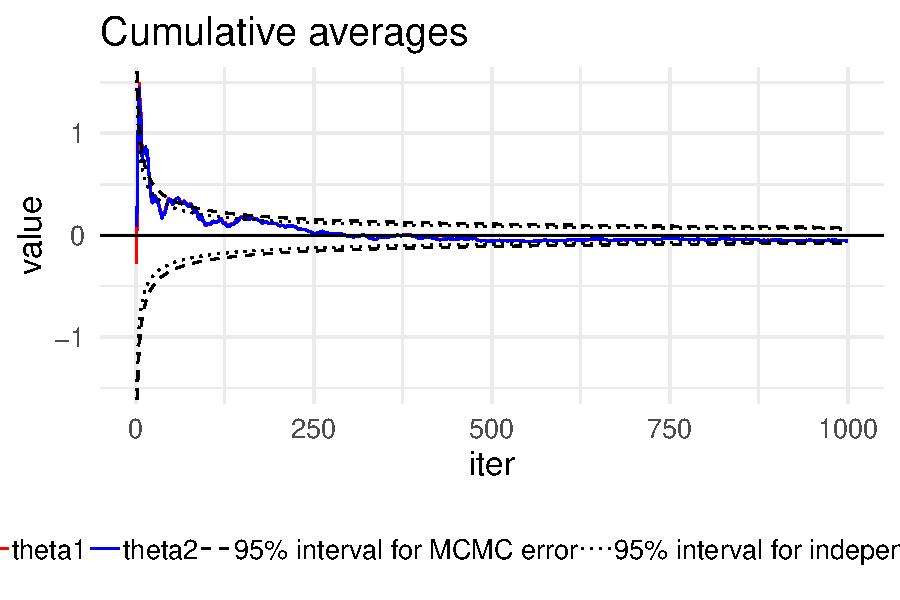
\includegraphics[width=12cm]{hmc1mcerr.pdf}}
\end{frame}

\begin{frame}

  {\Large\color{navyblue} Hamiltonian Monte Carlo}

  \begin{itemize}
  \item Uses log density (negative log density is called energy)
  \item Uses gradient of log density for more efficient sampling
  \item Augments parameter space with momentum variables
  \item Simulation of Hamiltonian dynamics reduces random walk
    \begin{itemize}
    \item Explanation of HMC with black board
    \item \url{http://elevanth.org/blog/2017/11/28/build-a-better-markov-chain/}
    \end{itemize}
  \end{itemize}

\end{frame}

\begin{frame}

  {\Large\color{navyblue} Hamiltonian Monte Carlo}

  \begin{itemize}
  \item Uses gradient of log density for more efficient sampling
  \item Alternating dynamic simulation and sampling energy level 
  \item<2-> Parameters: step size, number of steps in each chain
  \item<3-> No U-Turn Sampling (NUTS) and dynamic HMC
    \begin{itemize}
    \item adaptively selects number of steps to improve robustness and
      efficiency
    \item dynamic HMC refers to dynamic trajectory length
    \item to keep reversibility of Markov chain, need to simulate in two directions
    \item {\footnotesize \url{http://elevanth.org/blog/2017/11/28/build-a-better-markov-chain/}}
    \end{itemize}
  \item<4-> Dynamic simulation is discretized
    \begin{itemize}
    \item small step size gives accurate simulation, but requires more log density evaluations
    \item large step size reduces computation, but increases
      simulation error which needs to be taken into account in the
      Markov chain
    \item black board explanation of the effect of step size
    \end{itemize}
\end{itemize}

\end{frame}

\begin{frame}

  {\Large\color{navyblue} Adaptive dynamic HMC in Stan}

  \begin{itemize}
  \item Dynamic HMC using growing tree to increase simulation
    trajectory until no-U-turn criterion stopping
    \begin{itemize}
    \item max treedepth to keep computation in control
    \item<2-> pick a draw along the trajectory with probabilities adjusted
      to take into account the error in the discretized dynamic
      simulation
    \item<3-> give bigger weight for treeparts further away to increase
      probability of jumping further away
    \end{itemize}
  \item<4-> Mass matrix and step size adaptation in Stan
    \begin{itemize}
    \item<4-> mass matrix refers to having different scaling for different
      parameters and optionally also rotation to reduce correlations
    \item<5-> mass matrix and step size adjustment and are estimated
      during initial adaptation phase
    \item<6-> step size is adjusted to be as big as possible while keeping
      discretization error in control (adapt\_delta)
    \end{itemize}
  \item<7-> After adaptation the algorithm parameters are fixed
  \item<8-> After warmup store iterations for inference
  \item<9-> See more details in Stan reference manual
\end{itemize}

\end{frame}

\begin{frame}
  
  {\Large\color{navyblue} Max tree depth diagnostic}

  \begin{itemize}
  \item Dynamic HMC specific diagnostic
  \item Indicates inefficiency in sampling leading to higher
    autocorrelations and lower ESS ($n_{\rm eff}$)
  \item Different parameterizations matter
  \end{itemize}
\end{frame}


\begin{frame}
  
  {\Large\color{navyblue} Divergences}

  \begin{itemize}
  \item HMC specific: indicates that Hamiltonian dynamic simulation
    has problems with unexpected fast changes in log-density
    \begin{itemize}
    \item indicates possibility of biased estimates
    \end{itemize}
  \item Different parameterizations matter
  \item {\small \url{http://mc-stan.org/users/documentation/case-studies/divergences_and_bias.html}}
     \only<1>{\phantom{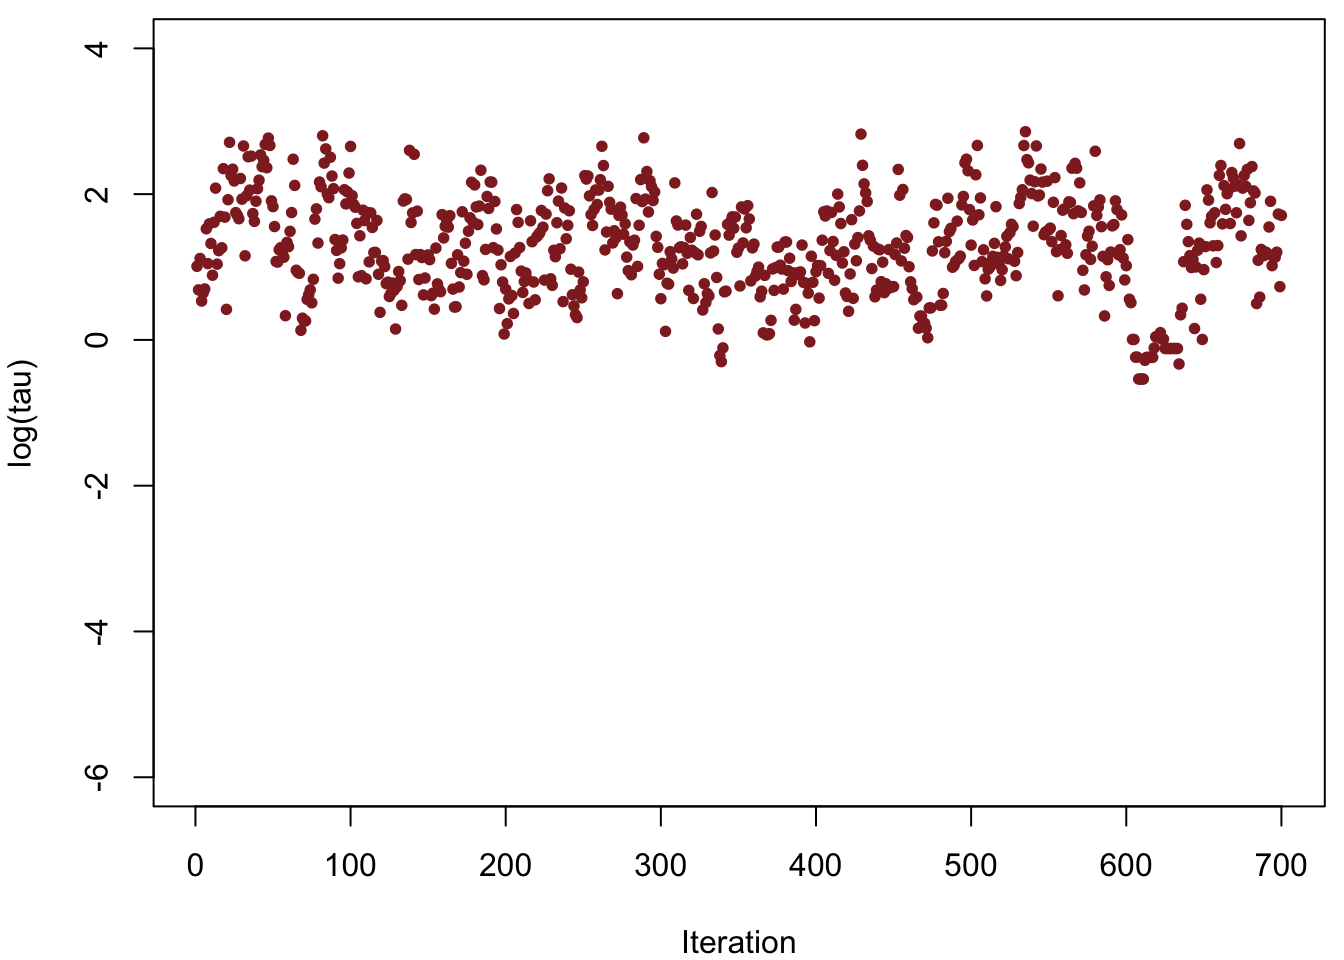
\includegraphics[width=8cm]{unnamed-chunk-6-1.png}}}
     \only<2>{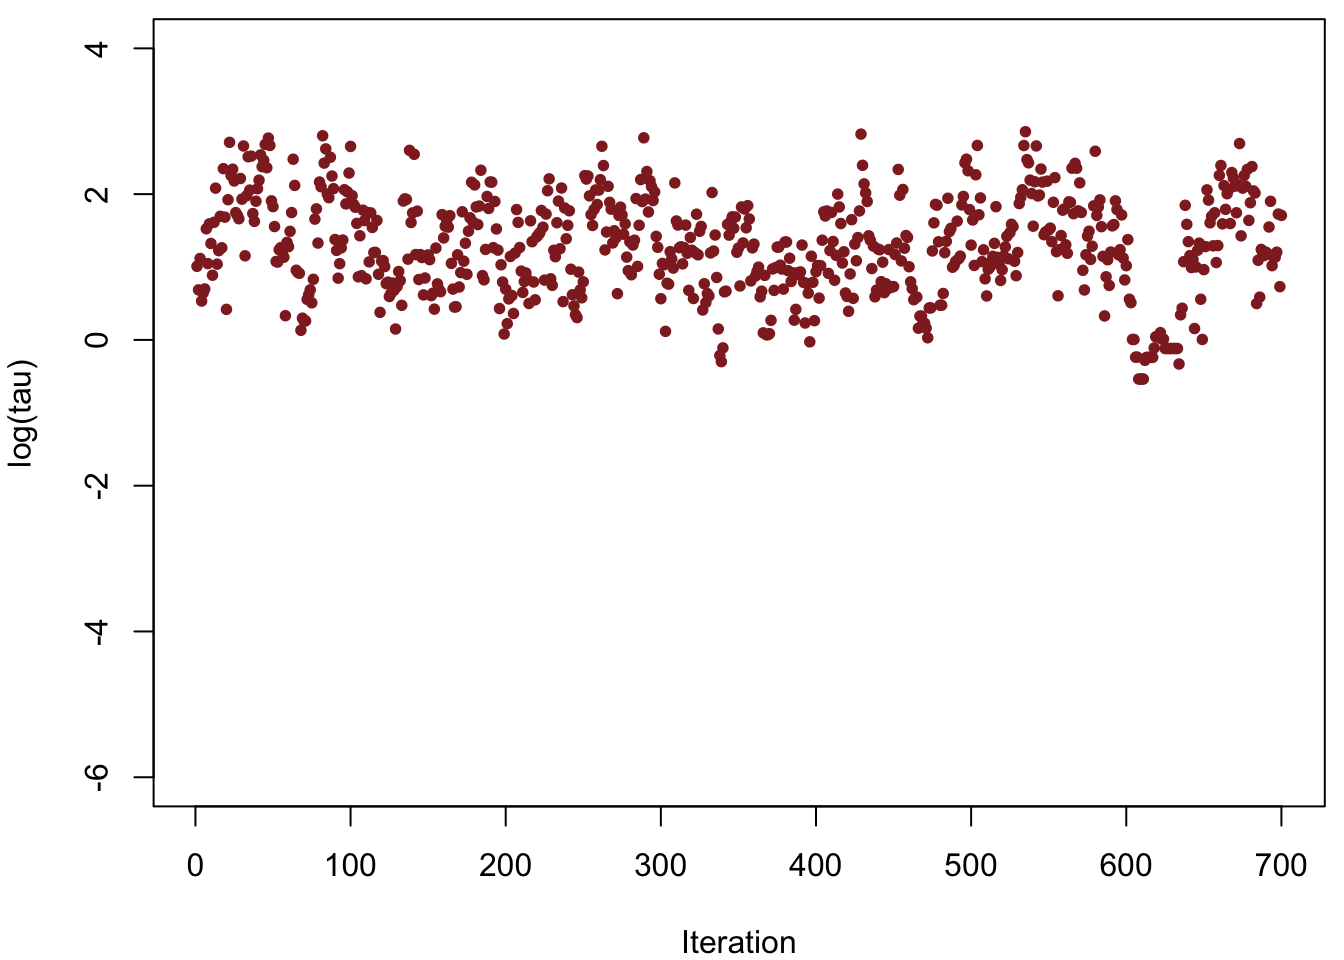
\includegraphics[width=8cm]{unnamed-chunk-6-1.png}}
     \only<3>{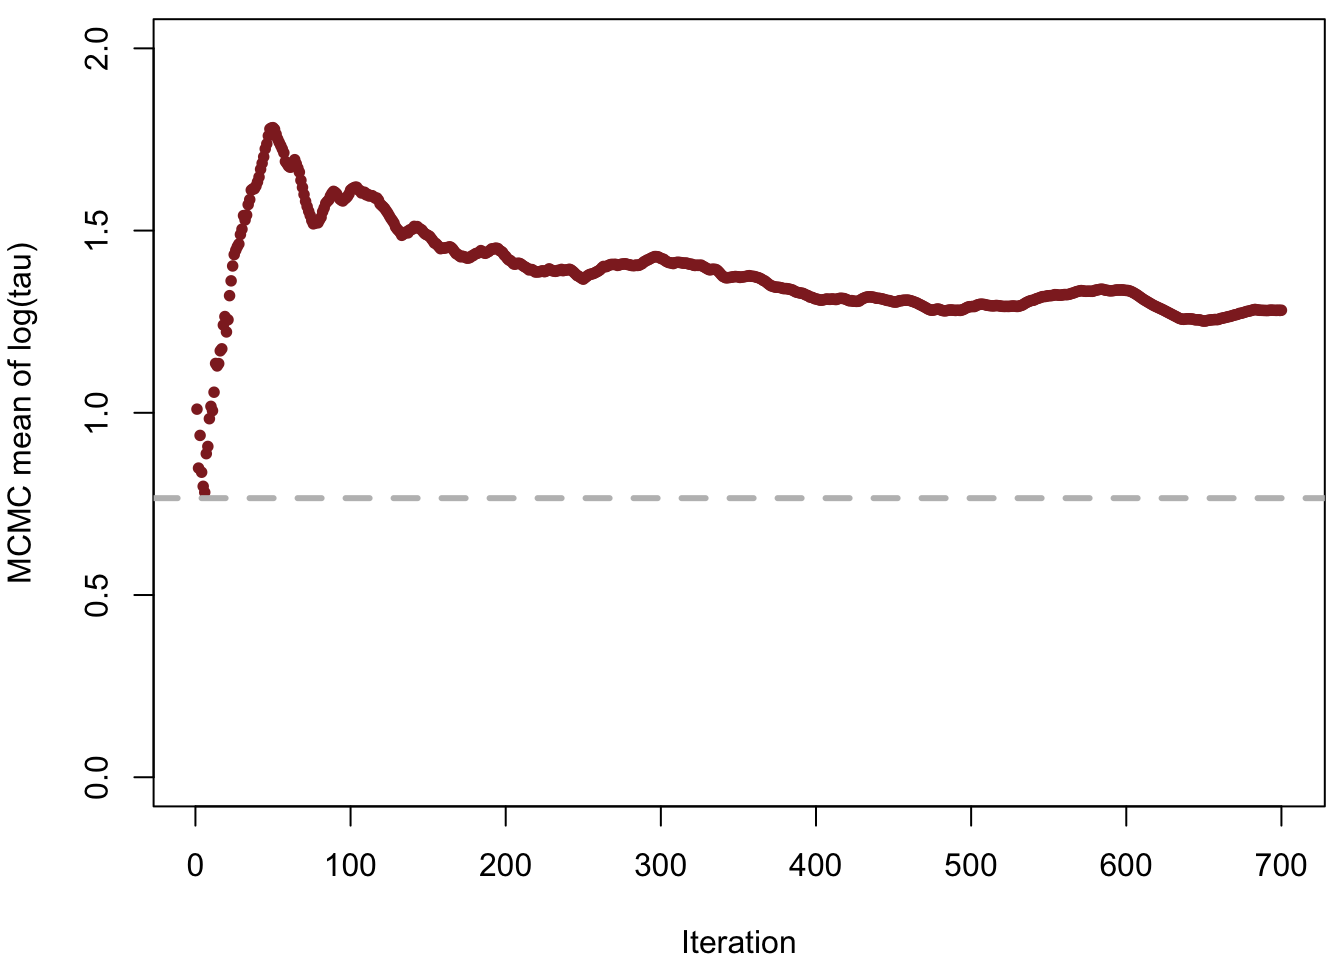
\includegraphics[width=8cm]{unnamed-chunk-7-1.png}}
     \only<4>{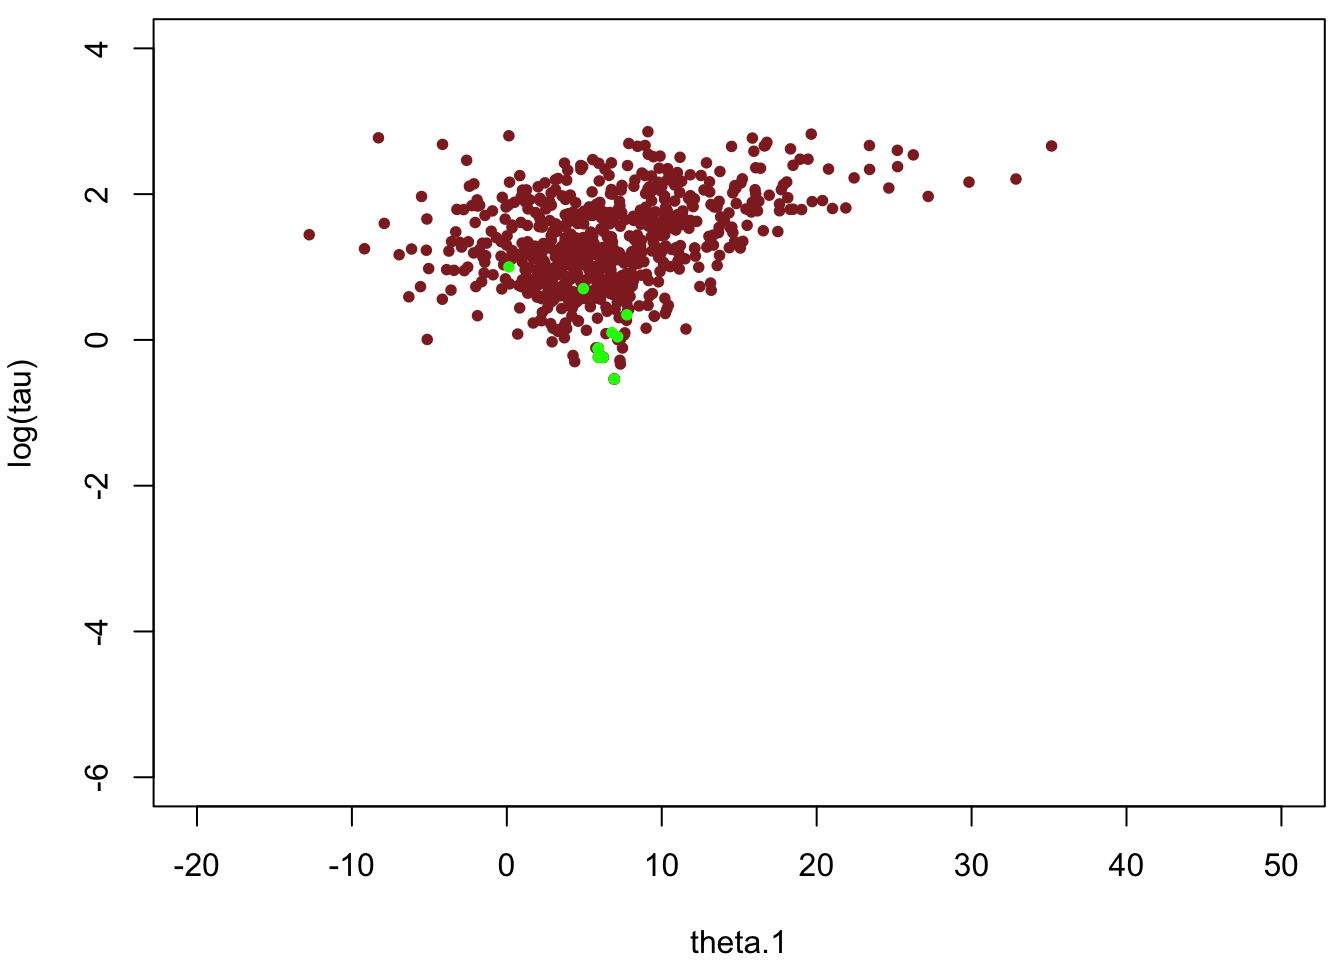
\includegraphics[width=8cm]{unnamed-chunk-9-1.png}}
     \only<5>{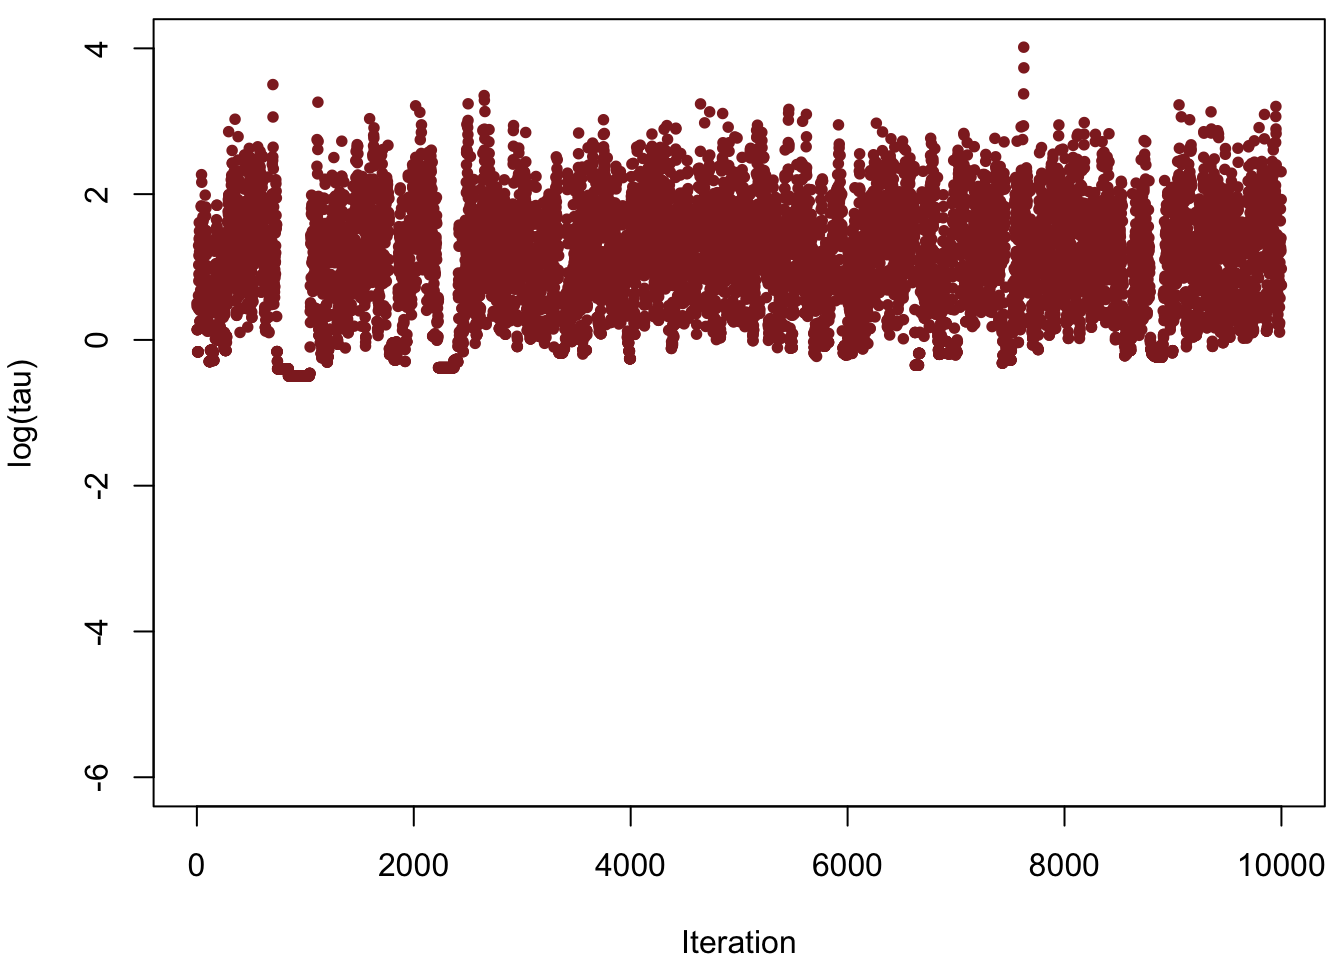
\includegraphics[width=8cm]{unnamed-chunk-12-1.png}}
     \only<6>{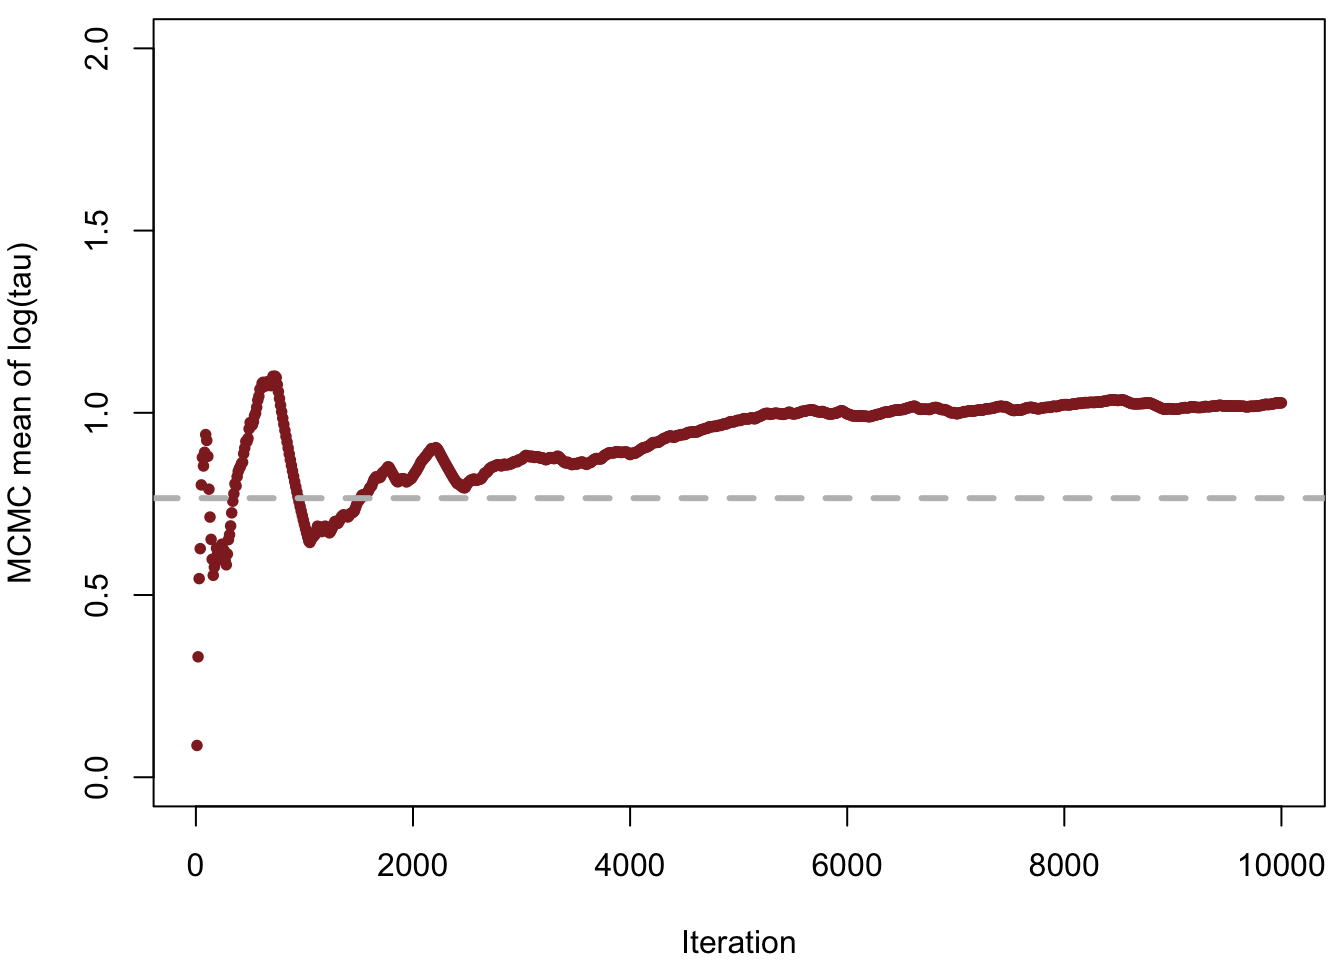
\includegraphics[width=8cm]{unnamed-chunk-13-1.png}}
     \only<7>{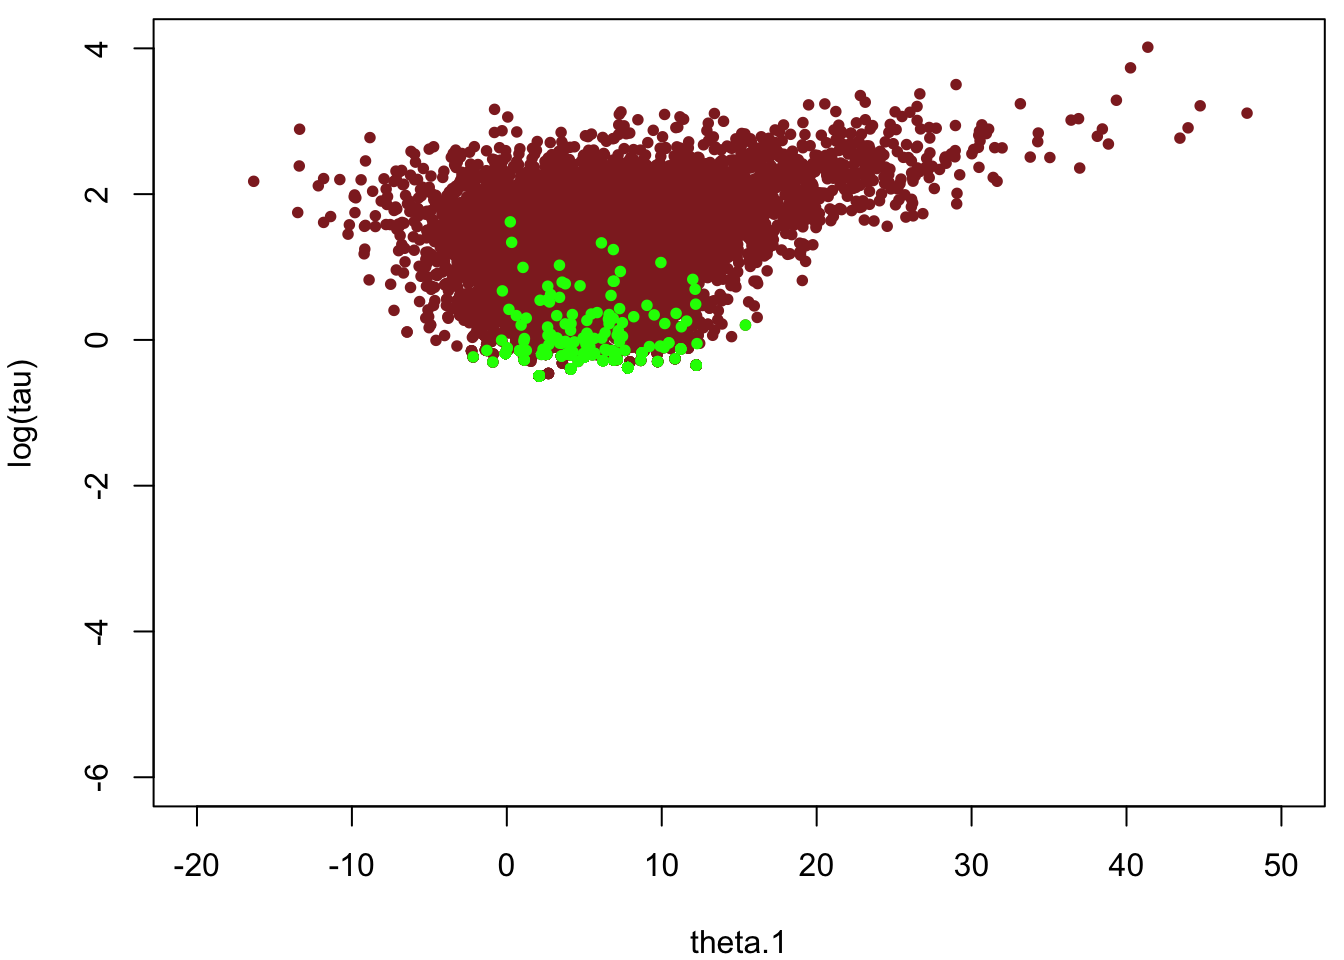
\includegraphics[width=8cm]{unnamed-chunk-15-1.png}}
     \only<8>{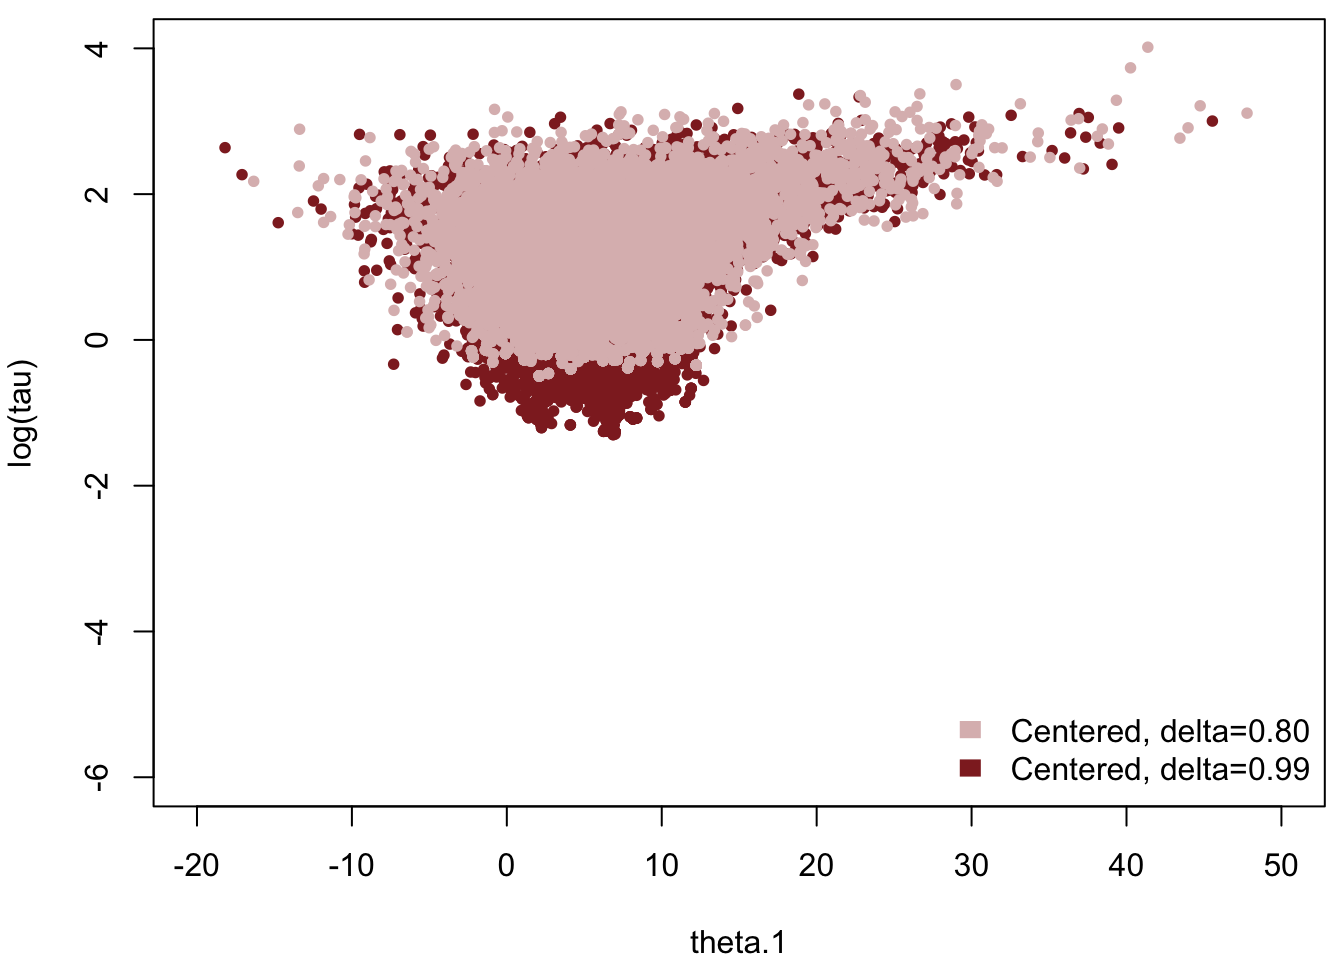
\includegraphics[width=8cm]{unnamed-chunk-21-1.png}}
     \only<9>{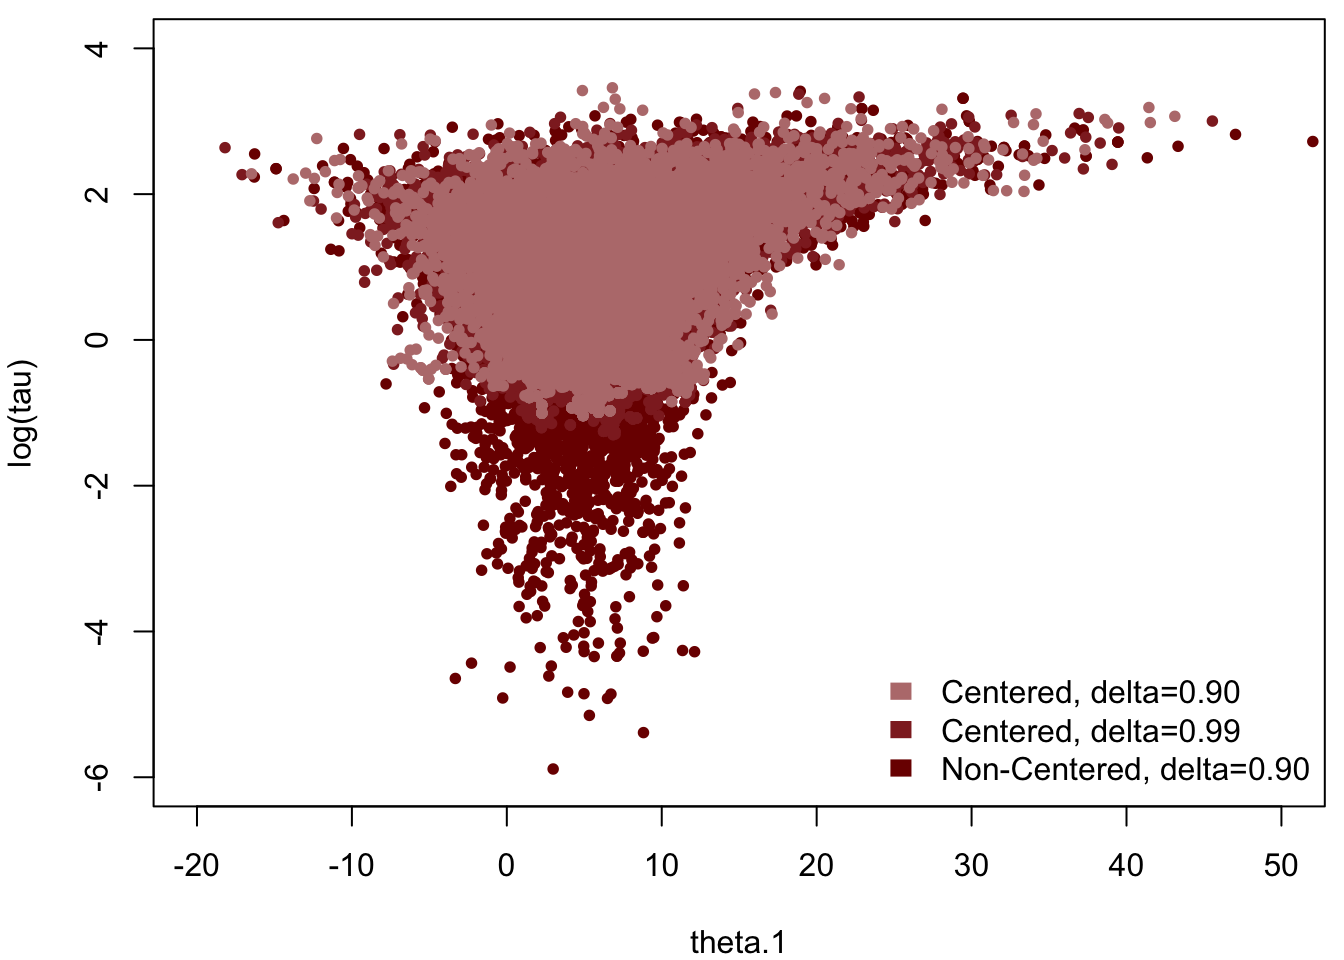
\includegraphics[width=8cm]{unnamed-chunk-31-1.png}}
  \end{itemize}
\end{frame}

\begin{frame}

  {\Large\color{navyblue} Problematic distributions}

  \begin{itemize}
  \item<1-> Nonlinear dependencies
    \begin{itemize}
    \item simple mass matrix scaling doesn't help
    \end{itemize}
  \item<2-> Funnels
    \begin{itemize}
    \item optimal step size depends on location
    \end{itemize}
  \item<3-> Multimodal
    \begin{itemize}
    \item difficult to move from one mode to another
    \end{itemize}
  \item<4-> Long-tailed with non-finite variance and mean
    \begin{itemize}
    \item effciency of exploration is reduced
    \item central limit theorem doesn't hold for mean and variance
    \end{itemize}
  \end{itemize}

\end{frame}

\begin{frame}

  {\Large\color{navyblue} Probabilistic programming language}
  
  \begin{itemize}
  \item Wikipedia ``A probabilistic programming language (PPL) is a
    programming language designed to describe probabilistic models
    and then perform inference in those models''
    \pause
  \item To make probabilistic programming useful
    \begin{itemize}
    \item inference has to be as automatic as possible
    \item diagnostics for telling if the automatic inference doesn't work
    \item easy workflow (to reduce manual work)
    \item fast enough (manual work replaced with automation)
    \end{itemize}
  \end{itemize}
\end{frame}

\begin{frame}
  
  {\Large\color{navyblue} Probabilistic programming}
  
  \begin{itemize}
  \item Enables agile workflow for developing probabilistic models
    \begin{itemize}
    \item language
    \item automated inference
    \item diagnostics
    \end{itemize}
  \item Many frameworks
    Stan, PyMC3, Pyro (Uber), Edward (Google), Birch, ELFI, ...
  \end{itemize}
  
\end{frame}

\begin{frame}

    {\Large\color{navyblue} Stan - probabilistic programming framework}

   \begin{itemize}
   \item Language, inference engine, user interfaces, documentation,
     case studies, diagnostics, packages, ...
     \begin{itemize}
     \item autodiff to compute gradients of the log density
     \end{itemize}
   \item<2-> More than ten thousand users in social, biological, and
     physical sciences, medicine, engineering, and business
     
   \item<3-> Several full time developers, 38 in dev team, more than 100 contributors
   \item<4-> R, Python, Julia, Scala, Stata, Matlab, command line interfaces
    \item<4-> More than 100 R packages using Stan
   \end{itemize}
  \vfill
  \begin{center}
    
\includegraphics[width=1.5cm]{stan_logo_wide.png}\\
    \url{mc-stan.org}
  \end{center}
\end{frame}

\begin{frame} 

  {\Large\color{navyblue} Stan}

  \begin{itemize}
  \item Stanislaw Ulam (1909-1984)
    \begin{itemize}
    \item Monte Carlo method
    \item H-Bomb
    \end{itemize}
  \end{itemize}
  
\end{frame}

\begin{frame}[fragile]

  {\Large\color{navyblue} Binomial model - Stan code}
  {\small\color{gray}
{\only<1>{\color{black}}
  \begin{lstlisting}[language=Stan]
data {
  int<lower=0> N;     // number of experiments
  int<lower=0,upper=N> y; // number of successes
}
\end{lstlisting}}
  {\only<2>{\color{black}}
\begin{lstlisting}[language=Stan]
parameters {
  real<lower=0,upper=1> theta; // parameter of the binomial
}
\end{lstlisting}}
{\only<3>{\color{black}}
\begin{lstlisting}[language=Stan]
model {
  theta ~ beta(1,1);     //prior
  y ~ binomial(N,theta); // observation model
}
\end{lstlisting}
}}
\end{frame} 

\begin{frame}[fragile]

  {\Large\color{navyblue} Binomial model - Stan code}
  
  {\small
  \begin{lstlisting}[language=Stan]
data {
  int<lower=0> N;     // number of experiments
  int<lower=0,upper=N> y; // number of successes
}
\end{lstlisting}}

  \begin{itemize}
  \item Data type and size are declared
  \item Stan checks that given data matches type and constraints
    \begin{itemize}
    \item<2-> If you are not used to strong typing, this may
      feel annoying, but it will reduce the probability of coding
      errors, which will reduce probability of data analysis errors
    \end{itemize}
  \end{itemize}
\end{frame}


\begin{frame}[fragile]

  {\Large\color{navyblue} Binomial model - Stan code}

  {\small
\begin{lstlisting}[language=Stan]
parameters {
  real<lower=0,upper=1> theta;
}
\end{lstlisting}}

  \begin{itemize}
  \item Parameters may have constraints
  \item Stan makes transformation to unconstrained space and samples in unconstrained space
    \begin{itemize}
    \item e.g. log transformation for <lower=a> 
    \item e.g. logit transformation for <lower=a,upper=b> 
    \end{itemize}
  \item<2-> For these declared transformation Stan automatically takes
    into account the Jacobian of the transformation (see BDA3 p. 21)
  \end{itemize}
\end{frame}

\begin{frame}[fragile]

  {\Large\color{navyblue} Binomial model - Stan code}
  
  {\small
\begin{lstlisting}[language=Stan]
model {
  theta ~ beta(1,1);     // prior
  y ~ binomial(N,theta); // likelihood
}
\end{lstlisting}}

\end{frame} 

\begin{frame}[fragile]

  {\Large\color{navyblue} Binomial model - Stan code}
  
  {\small
\begin{lstlisting}[language=Stan]
model {
  theta ~ beta(1,1);     // prior
  y ~ binomial(N,theta); // likelihood
}
\end{lstlisting}}

    \vspace{-0.5\baselineskip}
    \begin{itemize}
    \item $\sim$ is syntactic sugar and this is equivalent to
    \end{itemize}

  {\small
\begin{lstlisting}[language=Stan]
model {
  target += beta_lpdf(theta | 1, 1);
  target += binomial_lpmf(y | N, theta);
}
\end{lstlisting}}

    \vspace{-0.5\baselineskip}
    \begin{itemize}
    \item<2-> {\tt target} is the log posterior density
    \item<3-> {\tt \_lpdf} for continuous, {\tt \_lpmf} for discrete distributions (discrete for the left hand side of {\tt |})
    \item<4-> for Stan sampler there is no difference between prior and likelihood, all that matters is the final {\tt target}
    \item<5-> you can write in Stan language any program to compute the
      log density (Stan language is Turing complete)
    \end{itemize}

\end{frame} 

% \begin{frame}[fragile]

%   {\Large\color{navyblue} Binomial model - Stan code}
  
%   {\small
% \begin{lstlisting}[language=Stan]
% model {
%   theta ~ beta(1,1);     //prior
%   y ~ binomial(N,theta); // observation model
% }
% \end{lstlisting}}

%     \begin{itemize}
%     \item $\sim$ is syntactic sugar and this could be also written as
%     \end{itemize}

%   {\small
% \begin{lstlisting}[language=Stan]
% model {
%   target +=  beta_lpdf(theta | 1, 1);
%   target +=  binomial_lpmf(y | N, theta);
% }
% \end{lstlisting}}

%     \begin{itemize}
%     \end{itemize}
    
% \end{frame}

\begin{frame}
  
  {\Large\color{navyblue} Stan}
  
  \begin{itemize}
  \item Stan compiles (transplies) the model written in Stan language to C++
    \begin{itemize}
    \item this makes the sampling for complex models and bigger data faster
    \item also makes Stan models easily portable, you can use your own
      favorite interface
    \end{itemize}
  \end{itemize}

\end{frame}

\begin{frame}[fragile]

  {\Large\color{navyblue} RStan}

  {\small\color{gray}
    {\only<1>{\color{black}}
      RStan
\begin{lstlisting}[language=R]
library(rstan) 
rstan_options(auto_write = TRUE)
options(mc.cores = parallel::detectCores())
source('stan_utility.R')
\end{lstlisting}
    }
{\only<2>{\color{black}}
\begin{lstlisting}[language=R]
d_bin <- list(N = 10, y = 7)
fit_bin <- stan(file = 'binom.stan', data = d_bin)
\end{lstlisting}
}
}
\end{frame}

\begin{frame}[fragile]

  {\Large\color{navyblue} PyStan}

  {\small\color{gray}
{\only<1>{\color{black}}
      PyStan
\begin{lstlisting}
import pystan
import stan_utility
\end{lstlisting}
    }
    {\only<2>{\color{black}}
\begin{lstlisting}
data = dict(N=10, y=8)
model = stan_utility.compile_model('binom.stan')
fit = model.sampling(data=data)
\end{lstlisting}
    }
  }
\end{frame}

\begin{frame}

  {\Large\color{navyblue} Stan}
  
  \begin{itemize}
  \item Compilation (unless previously compiled model available)
  \item Warm-up including adaptation
  \item Sampling
  \item Generated quantities
  \item Save posterior draws
  \item Report divergences, $n_\eff$, $\widehat{R}$
  \end{itemize}

\end{frame}

\begin{frame}[fragile]

  {\Large\color{navyblue} Difference between proportions}
  
\begin{itemize}
  \item An experiment was performed to estimate the effect of
    beta-blockers on mortality of cardiac patients
  \item A group of
    patients were randomly assigned to treatment and control groups:
    \begin{itemize}
    \item out of 674 patients receiving the control, 39 died
    \item out of 680 receiving the treatment, 22 died
    \end{itemize}
  \end{itemize}
\end{frame}

\begin{frame}[fragile]

  {\Large\color{navyblue} Difference between proportions}

%  Beta-blockers $N_1 = 674, y_1 = 39, N_2 = 680, y_2 = 22$
  
  {\small\color{gray}
    {\only<1>{\color{black}}
\begin{lstlisting}[language=Stan]
data {
  int<lower=0> N1;
  int<lower=0> y1;
  int<lower=0> N2;
  int<lower=0> y2;
}
parameters {
  real<lower=0,upper=1> theta1;
  real<lower=0,upper=1> theta2;
}
model {
  theta1 ~ beta(1,1);
  theta2 ~ beta(1,1);
  y1 ~ binomial(N1,theta1);
  y2 ~ binomial(N2,theta2);
}
\end{lstlisting}
    }
    {\only<2>{\color{black}}
\begin{lstlisting}[language=Stan]
generated quantities {
  real oddsratio;
  oddsratio = (theta2/(1-theta2))/(theta1/(1-theta1));
}
\end{lstlisting}
    }
  }
\end{frame}

\begin{frame}[fragile]

  {\Large\color{navyblue} Difference between proportions}

%  Beta-blockers $N_1 = 674, y_1 = 39, N_2 = 680, y_2 = 22$
  
  {\small
\begin{lstlisting}[language=Stan]
generated quantities {
  real oddsratio;
  oddsratio = (theta2/(1-theta2))/(theta1/(1-theta1));
}
\end{lstlisting}
    }

    \begin{itemize}
    \item generated quantities is run after the sampling
    \end{itemize}
    
\end{frame}

\begin{frame}[fragile]

  {\Large\color{navyblue} Difference between proportions}
  
  {\small
\begin{lstlisting}[language=R]
d_bin2 <- list(N1 = 674, y1 = 39, N2 = 680, y2 = 22)
fit_bin2 <- stan(file = 'binom2.stan', data = d_bin2)
\end{lstlisting}
  }

  {\tiny
\begin{lstlisting}
starting worker pid=10151 on localhost:11783 at 10:03:27.872
starting worker pid=10164 on localhost:11783 at 10:03:28.087
starting worker pid=10176 on localhost:11783 at 10:03:28.295
starting worker pid=10185 on localhost:11783 at 10:03:28.461

SAMPLING FOR MODEL 'binom2' NOW (CHAIN 1).

Gradient evaluation took 6e-06 seconds
1000 transitions using 10 leapfrog steps per transition would take 0.06 seconds.
Adjust your expectations accordingly!


Iteration:    1 / 2000 [  0%]  (Warmup)
Iteration:  200 / 2000 [ 10%]  (Warmup)
...
Iteration: 1000 / 2000 [ 50%]  (Warmup)
Iteration: 1001 / 2000 [ 50%]  (Sampling)
...
Iteration: 2000 / 2000 [100%]  (Sampling)

 Elapsed Time: 0.012908 seconds (Warm-up)
               0.017027 seconds (Sampling)
               0.029935 seconds (Total)


SAMPLING FOR MODEL 'binom2' NOW (CHAIN 2).
...
\end{lstlisting}
  }

\end{frame}

\begin{frame}[fragile]

  {\Large\color{navyblue} Difference between proportions}
  
  {\small
\begin{lstlisting}[language=R]
monitor(fit_bin2, probs = c(0.1, 0.5, 0.9))
\end{lstlisting}
  }

  {\scriptsize
\begin{lstlisting}
Inference for the input samples 
(4 chains: each with iter=1000; warmup=0):

            mean se_mean  sd    10%    50%    90% n_eff Rhat
theta1       0.1       0 0.0    0.0    0.1    0.1  3280    1
theta2       0.0       0 0.0    0.0    0.0    0.0  3171    1
oddsratio    0.6       0 0.2    0.4    0.6    0.8  3108    1
lp__      -253.5       0 1.0 -254.8 -253.2 -252.6  1922    1

For each parameter, n_eff is a crude measure of effective sample size,
and Rhat is the potential scale reduction factor on split chains (at 
convergence, Rhat=1).
\end{lstlisting}
  }

  \begin{itemize}
  \item<2-> {\tt lp\_\_} is the log density, ie, same as {\tt target}
  \end{itemize}
  
\end{frame}

\begin{frame}[fragile]

  {\Large\color{navyblue} Difference between proportions}
  
  {\small
\begin{lstlisting}
draws <- as.data.frame(fit_bin2)
mcmc_hist(draws, pars = 'oddsratio') +
  geom_vline(xintercept = 1) +
  scale_x_continuous(breaks = c(seq(0.25,1.5,by=0.25)))
\end{lstlisting}
  }

  \begin{center}
  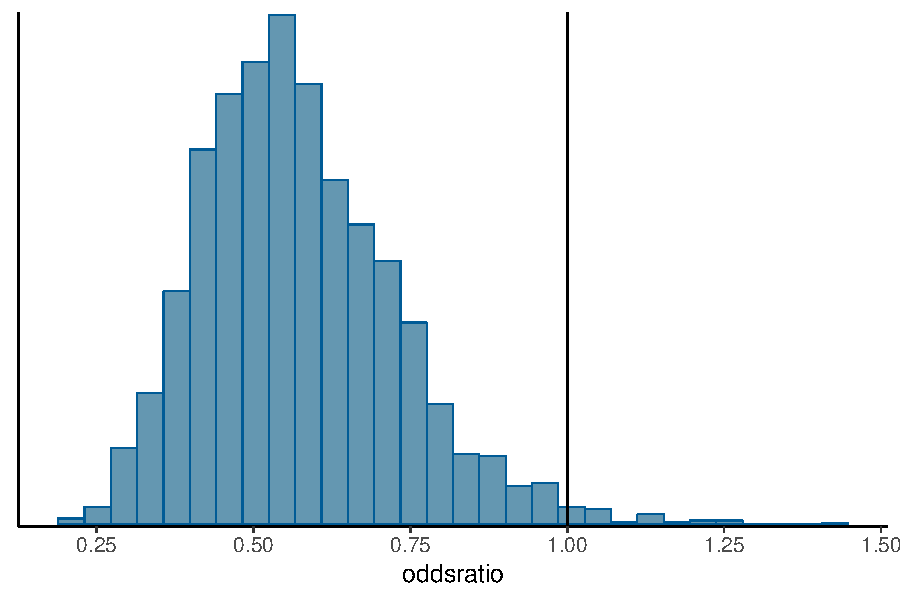
\includegraphics[width=9cm]{betablockoddsratio.pdf}
\end{center}
\end{frame}


\begin{frame}[fragile]

  {\Large\color{navyblue} HMC specific diagnostics}
  
  {\scriptsize
\begin{lstlisting}
check_treedepth(fit_bin2)
check_energy(fit_bin2)
check_div(fit_bin2)

[1] "0 of 4000 iterations saturated the maximum tree depth of 10 (0%)"
[1] "0 of 4000 iterations ended with a divergence (0%)"
\end{lstlisting}
  }
  
\end{frame}
  
\begin{frame}[fragile]

  {\Large\color{navyblue} Shinystan}

  \begin{itemize}
  \item Graphical user interface for analysing MCMC results
  \end{itemize}
  
\end{frame} 

\begin{frame}

  {\Large\color{navyblue} Kilpisjärvi summer temperature}
  
  \begin{itemize}
  \item Temperature at Kilpisjärvi in June, July and August from 1952 to 2013
  \item Is there change in the temperature?
  \end{itemize}
  \begin{center}
    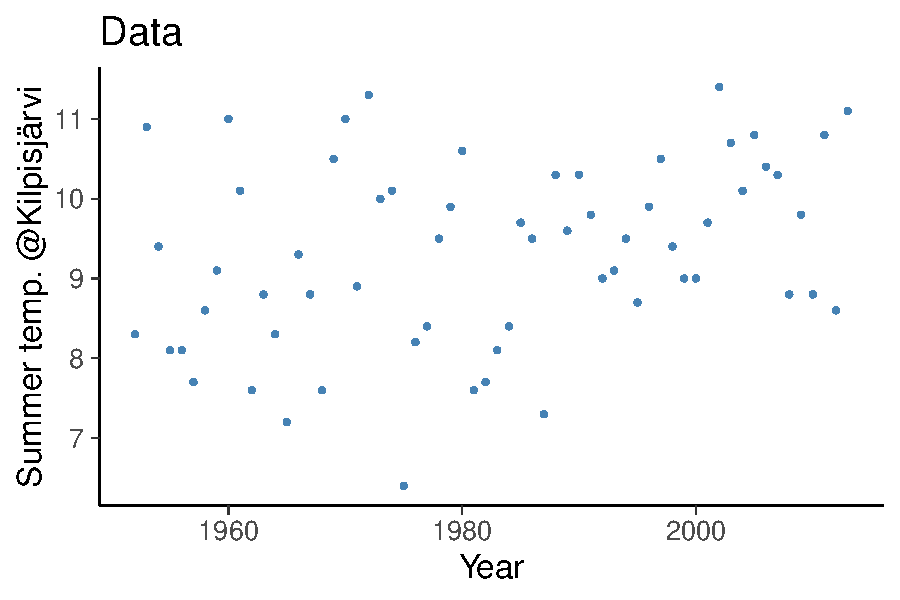
\includegraphics[width=10cm]{kilpis_data.pdf}
  \end{center}
  
\end{frame}

\begin{frame}[fragile]

  {\Large\color{navyblue} Gaussian linear model}
  {\small
  \begin{lstlisting}[language=Stan]
data {
    int<lower=0> N; // number of data points 
    vector[N] x; // 
    vector[N] y; // 
}
parameters {
    real alpha; 
    real beta; 
    real<lower=0> sigma;
}
transformed parameters {
    vector[N] mu;
    mu <- alpha + beta*x;
}
model {
    y ~ normal(mu, sigma);
}
  \end{lstlisting}
}
\end{frame} 

\begin{frame}[fragile]

  {\Large\color{navyblue} Gaussian linear model}
  {\small
  \begin{lstlisting}[language=Stan]
data {
    int<lower=0> N; // number of data points 
    vector[N] x; // 
    vector[N] y; // 
}
\end{lstlisting}
  }

  \begin{itemize}
  \item difference between {\tt vector[N] x}\, and\, {\tt real x[N]}
  \end{itemize}
\end{frame}

\begin{frame}[fragile]

  {\Large\color{navyblue} Gaussian linear model}
  {\small
  \begin{lstlisting}[language=Stan]
    parameters {
    real alpha; 
    real beta; 
    real<lower=0> sigma;
}
transformed parameters {
    vector[N] mu;
    mu <- alpha + beta*x;
}
\end{lstlisting}
  }
  \begin{itemize}
  \item transformed parameters are deterministic transformations of parameters and data
  \end{itemize}
\end{frame} 

\begin{frame}[fragile]

  {\Large\color{navyblue} Priors for Gaussian linear model}
  {\small
  \begin{lstlisting}[language=Stan]
data {
    int<lower=0> N; // number of data points 
    vector[N] x; // 
    vector[N] y; // 
    real pmualpha; // prior mean for alpha
    real psalpha;  // prior std for alpha
    real pmubeta;  // prior mean for beta
    real psbeta;   // prior std for beta
}
...
transformed parameters {
    vector[N] mu;
    mu <- alpha + beta*x;
}
model {
    alpha ~ normal(pmualpha,psalpha);
    beta ~ normal(pmubeta,psbeta);
    y ~ normal(mu, sigma);
}
  \end{lstlisting}
}
\end{frame} 

\begin{frame}[fragile]

  {\Large\color{navyblue} Student-t linear model}
  {\small
  \begin{lstlisting}[language=Stan]
...
parameters {
  real alpha; 
  real beta; 
  real<lower=0> sigma;
  real<lower=1,upper=80> nu;
}
transformed parameters {
  vector[N] mu;
  mu <- alpha + beta*x;
}
model {
  nu ~ gamma(2,0.1); 
  y ~ student_t(nu, mu, sigma);
}
  \end{lstlisting}
}
\end{frame} 

\begin{frame}
  
  {\Large\color{navyblue} Priors}

  \begin{itemize}
  \item Prior for temperature increase?
  \end{itemize}

\end{frame}

\begin{frame}

  {\Large\color{navyblue} Kilpisjärvi summer temperature}

  Posterior fit
  
  \begin{center}
    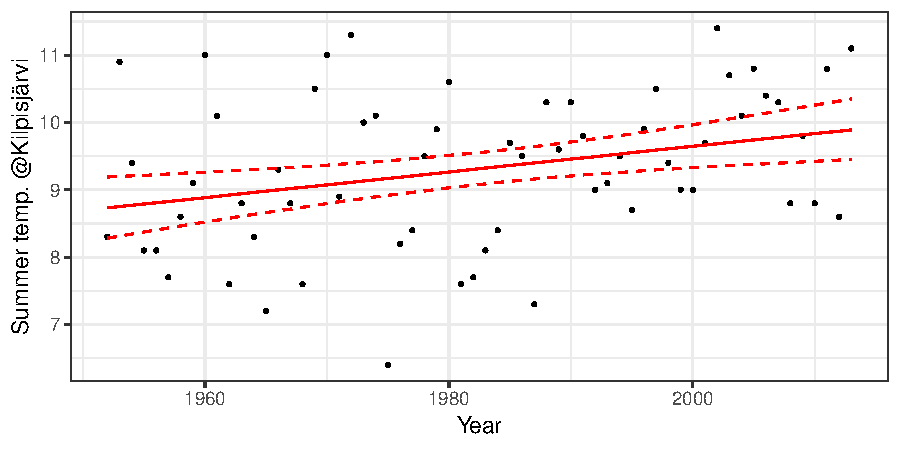
\includegraphics[width=10cm]{kilpis_lin_pfit.pdf}
  \end{center}

\end{frame}

\begin{frame}[fragile]

  {\Large\color{navyblue} Kilpisjärvi summer temperature}

  Posterior draws of alpha and beta
  
  \begin{center}
    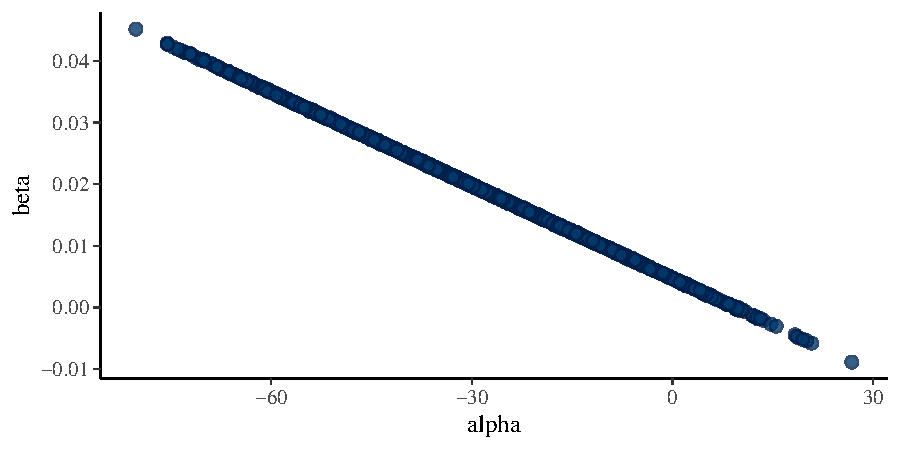
\includegraphics[width=10cm]{kilpis_lin_mcmc_scatter.pdf}
  \end{center}
 
\end{frame}

\begin{frame}[fragile]

  {\Large\color{navyblue} Kilpisjärvi summer temperature}
  
  Posterior draws of alpha and beta
  
  \begin{center}
    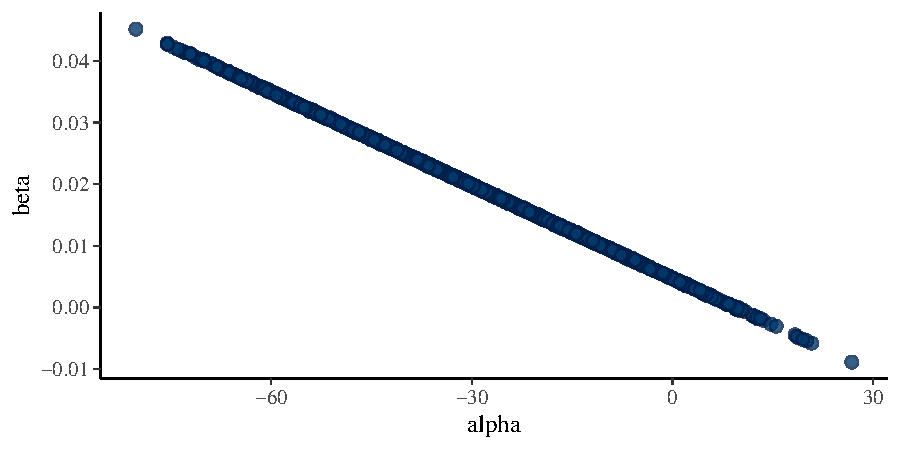
\includegraphics[width=10cm]{kilpis_lin_mcmc_scatter.pdf}
  \end{center}

{\scriptsize
\begin{lstlisting}
There were 14 transitions after warmup that exceeded the maximum
treedepth. Increase max_treedepth above 10. See 
http://mc-stan.org/misc/warnings.html#maximum-treedepth-exceeded
Examine the pairs() plot to diagnose sampling problems
\end{lstlisting}
}
  
\end{frame}

\begin{frame}[fragile]
  
  {\Large\color{navyblue} Linear regression model in Stan}
  
  {\scriptsize
\begin{lstlisting}[language=Stan]
data {
  int<lower=0> N; // number of data points
  vector[N] x; //
  vector[N] y; //
  real xpred; // input location for prediction
}
transformed data {
  vector[N] x_std;
  vector[N] y_std;
  real xpred_std;
  x_std = (x - mean(x)) / sd(x);
  y_std = (y - mean(y)) / sd(y);
  xpred_std = (xpred - mean(x)) / sd(x);
}
\end{lstlisting}
  }
\end{frame}

%XXXX add better posterior draws

\begin{frame}[fragile]

  {\Large\color{navyblue} RStanARM}

  \begin{itemize}
  \item RStanARM provides simplified model description with
    pre-compiled models
    \begin{itemize}
    \item no need to wait for compilation
    \item a restricted set of models
    \end{itemize}
  \end{itemize}

Two group Binomial model:
  {\scriptsize
\begin{lstlisting}
d_bin2 <- data.frame(N = c(674, 680), y = c(39,22), grp2 = c(0,1))
fit_bin2 <- stan_glm(y/N ~ grp2, family = binomial(), data = d_bin2,
                    weights = N)
\end{lstlisting}
  }
% \begin{lstlisting}[language=R]
% draws_bin2 <- as.data.frame(fit_bin2) %>%
%   mutate(theta1 = plogis(`(Intercept)`),
%          theta2 = plogis(`(Intercept)` + grp2),
%          oddsratio = (theta2/(1-theta2))/(theta1/(1-theta1)))

% mcmc_hist(draws_bin2, pars='oddsratio')
% \end{lstlisting}
%     }
    
\end{frame} 

\begin{frame}[fragile]

  {\Large\color{navyblue} RStanARM}

  \begin{itemize}
  \item RStanARM provides simplified model description with
    pre-compiled models
    \begin{itemize}
    \item no need to wait for compilation
    \item a restricted set of models
    \end{itemize}
  \end{itemize}

Two group Binomial model:
  {\scriptsize
\begin{lstlisting}
d_bin2 <- data.frame(N = c(674, 680), y = c(39,22), grp2 = c(0,1))
fit_bin2 <- stan_glm(y/N ~ grp2, family = binomial(), data = d_bin2,
                    weights = N)
\end{lstlisting}
  }
    Gaussian linear model
  {\scriptsize
\begin{lstlisting}
    fit_lin <- stan_glm(temp ~ year, data = d_lin)
\end{lstlisting}
  }
% \begin{lstlisting}[language=R]
% draws_bin2 <- as.data.frame(fit_bin2) %>%
%   mutate(theta1 = plogis(`(Intercept)`),
%          theta2 = plogis(`(Intercept)` + grp2),
%          oddsratio = (theta2/(1-theta2))/(theta1/(1-theta1)))

% mcmc_hist(draws_bin2, pars='oddsratio')
% \end{lstlisting}
%     }
    
\end{frame} 


\begin{frame}[fragile]

  {\Large\color{navyblue} BRMS}

  \begin{itemize}
  \item BRMS provides simplified model description
    \begin{itemize}
    \item a larger set of models than RStanARM, but still restricted
    \item need to wait for the compilation
    \end{itemize}
  \end{itemize}

  {\scriptsize
\begin{lstlisting}[language=R]
fit_bin2 <- brm(y/N ~ grp2, family = binomial(), data = d_bin2,
                    weights = N)


fit_lin_t <- brm(temp ~ year, data = d_lin, family = student())
\end{lstlisting}
    }
    
\end{frame} 

\begin{frame}

  {\Large\color{navyblue} Extreme value analysis}

Geomagnetic storms

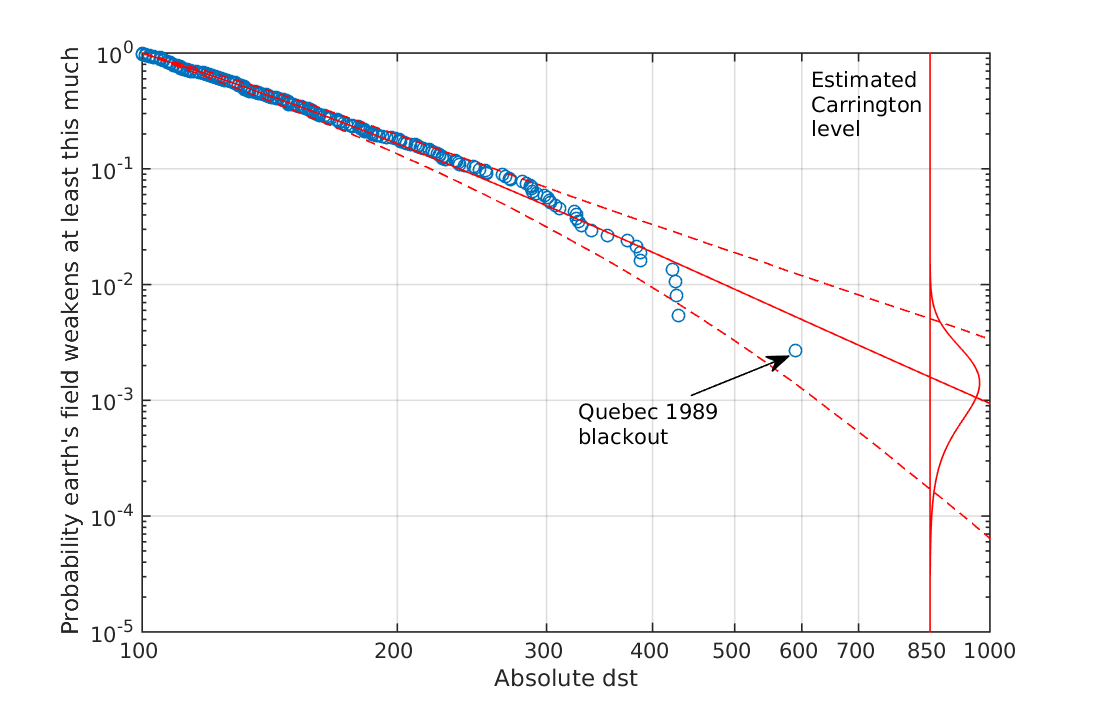
\includegraphics[width=12cm]{stan_gpareto_geomev.png}  

\end{frame}

\begin{frame}[fragile]

  {\Large\color{navyblue} Extreme value analysis}
  {\small
  \begin{lstlisting}[language=Stan]
data {
  int<lower=0> N;
  vector<lower=0>[N] y;
  int<lower=0> Nt;
  vector<lower=0>[Nt] yt;
}
transformed data {
  real ymax;
  ymax <- max(y);
}
parameters {
  real<lower=0> sigma; 
  real<lower=-sigma/ymax> k; 
}
model {
  y ~ gpareto(k, sigma);
}
generated quantities {
  vector[Nt] predccdf;
  predccdf<-gpareto_ccdf(yt,k,sigma);
}
  \end{lstlisting}
}
\end{frame} 

\begin{frame}[fragile]

  {\Large\color{navyblue} Functions}
  {\footnotesize
  \begin{lstlisting}[language=Stan]
functions {
  real gpareto_lpdf(vector y, real k, real sigma) {
    // generalised Pareto log pdf with mu=0
    // should check and give error if k<0 
    // and max(y)/sigma > -1/k
    int N;
    N <- dims(y)[1];
    if (fabs(k) > 1e-15)
      return -(1+1/k)*sum(log1pv(y*k/sigma)) -N*log(sigma);
    else
      return -sum(y/sigma) -N*log(sigma); // limit k->0
  }
  vector gpareto_ccdf(vector y, real k, real sigma) {
    // generalised Pareto log ccdf with mu=0
    // should check and give error if k<0 
    // and max(y)/sigma < -1/k
    if (fabs(k) > 1e-15)
      return exp((-1/k)*log1pv(y/sigma*k));
    else
      return exp(-y/sigma); // limit k->0
  }
}
  \end{lstlisting}
}
\end{frame} 



\begin{frame}[fragile]

  {\Large\color{navyblue} Other packages}

  \begin{itemize}
  \item R
    \begin{itemize}
    \item shinystan --- interactive diagnostics
    \item bayesplot --- visualization and model checking (see model checking in Ch 6)
    \item loo --- cross-validation model assessment, comparison and averaging (see Ch 7)
    \item projpred --- projection predictive variable selection
    \end{itemize}
    \vspace{\baselineskip}
  \item Python
    \begin{itemize}
    \item ArviZ --- visualization, and model checking and assessment (see Ch 6 and 7)
    \end{itemize}
  \end{itemize}

\end{frame} 

\end{document}

%%% Local Variables: 
%%% TeX-PDF-mode: t
%%% TeX-master: t
%%% End: 
